\documentclass{book}
\usepackage{graphicx,makeidx,textcomp,tipa,siunitx,tikz,multicol,hyperref}
\usepackage[utf8]{inputenc}
\usepackage[all]{hypcap}
\usepackage[normalem]{ulem}
\renewcommand{\thefootnote}{\fnsymbol{footnote}}
\pdfcompresslevel 9

\title{Eggshell / Plants}
\author{B M Corser}
\date{Janurary -- March 2013}

\begin{document}

\maketitle

\tableofcontents

\chapter{Nature Eruption}

\begin{figure}
\centering
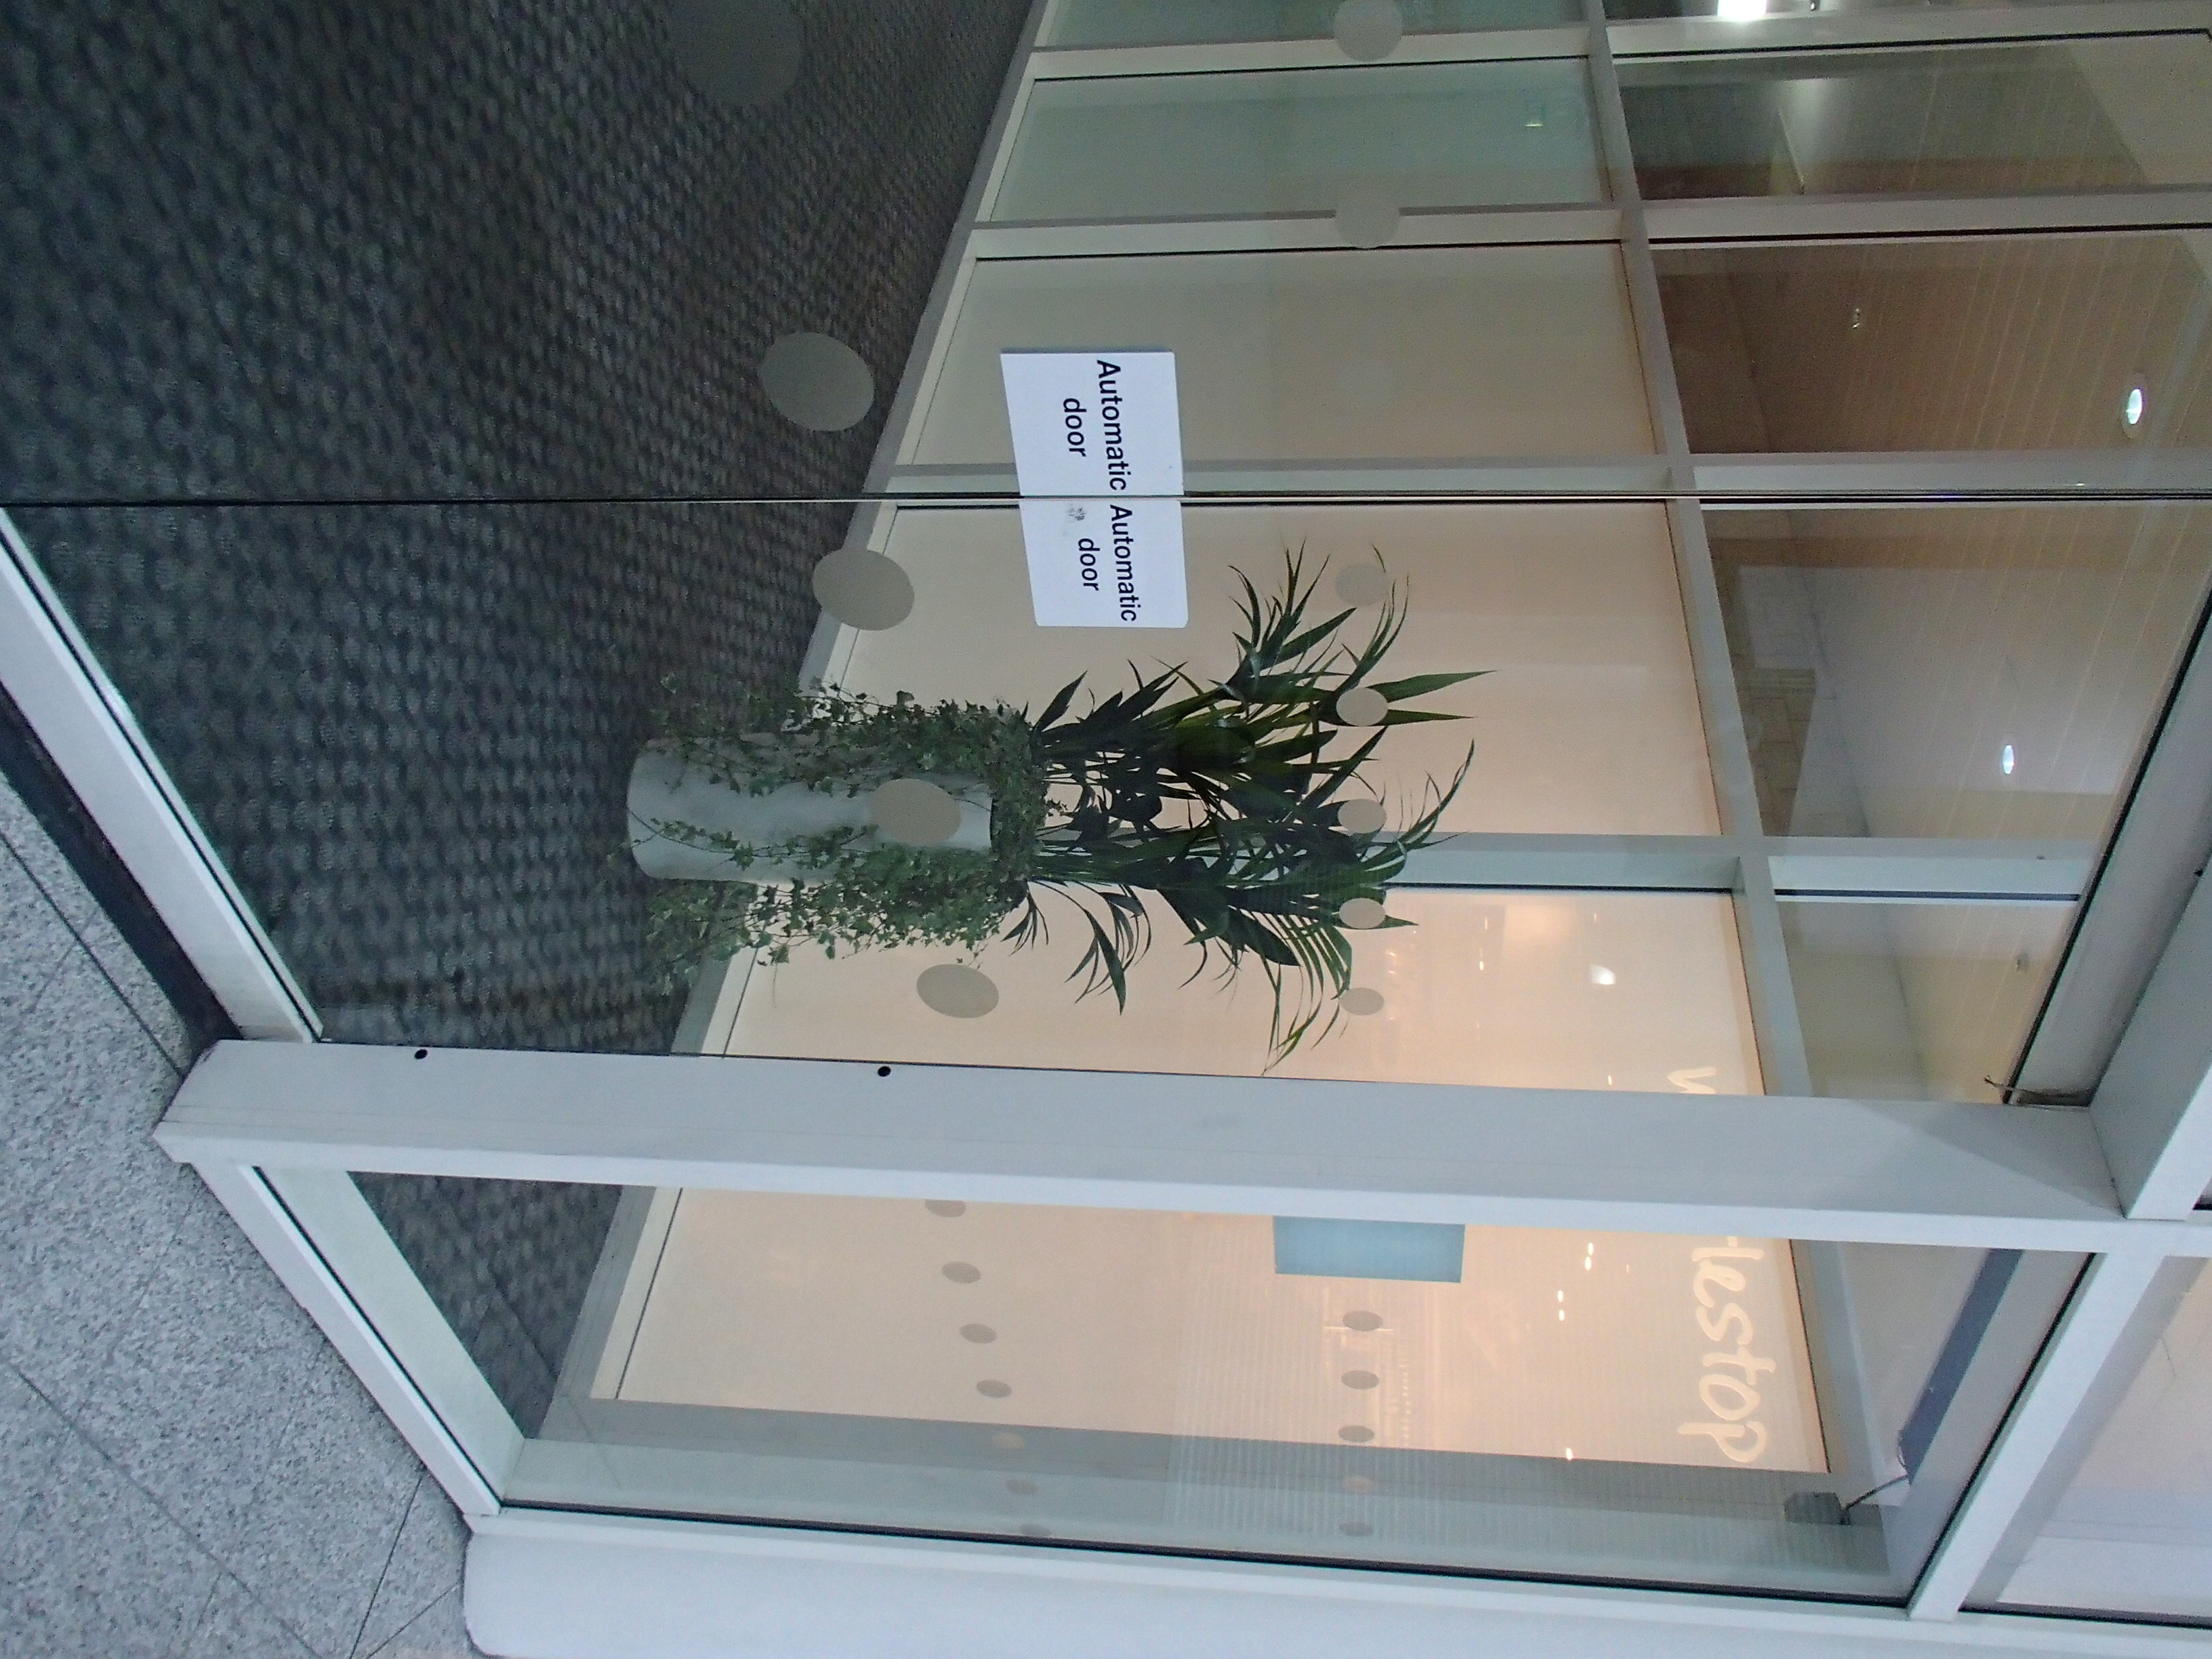
\includegraphics[width=\textwidth,angle=90]{figures/P1050140.JPG}
\caption{Nature Eruption}
\end{figure}

It is only in the quiet of panels, when horror vacui is quietly receded from,
that movement can begin to come from nature. A thing that should not shudder
begins to exhibit the first tremors of life. There is a sensation of bubbling
beneath the feet, a fibrous crunching, something like the tiny sounds at the
bottom of the lungs on a deep breath. There is a kind of panting. Surely an
eruption is coming.

In a regimented frame, there is an attempt to cast authority through the
appearance of order. This is a setting without exclamation. This is not a place
where anything slides luxuriously from upright to reclining, but a desperate
calmness sites itself in the air, an hyperactive stillness. It is not possible
to situate this frame (to give it a context or some kind of Gestalt backdrop),
instead an observer must attempt to impose herself as a figure for the things
she sees to stand a chance of approaching corporeality. This impetus is
well-anticipated in the viewer; a sturdy pastiche of their figure is ``pre''
placed in the scene, already there, waiting to be called into play by this
acknowledgement.

There is no pointed coquettishness or promise, instead there is an air of
hastily conceived urgency, like a dull ambient panic or pale anxiety. The
subtly implied threat of grey and misty Lacanian reality is veiled with an
extreme economy of gesture. As lightly as is is possible to contain something
is how things are contained here. It is impressive, then, that this containment
is able to be so utterly complete.

This should surely be the conception of a very sublime perspective, to solve an
issue outside of flesh and to have solved it with so light a touch. It is
difficult to see the weight (or power) that maintains the rigidity holding
things up.  This ``weight'' is hidden by design, stacked above head-height,
stuffed inside walls, mirrored away or disguised in large-scale optical
illusion.

There is a physical tension around us, it feels like being inside a cat's
cradle. This is not a situation that begs exploration. We explore anyway.

Free movement in this space makes the space itself feel tenuous. It is as if
the whole charade could wink out of existence if a certain or particular floor
tile were stepped on.  \emph{The three of us tread carefully.} We emulate the
stasis through which we find ourselves moving.

Right now, nothing suggests relief will come, the unbroken hush hums lulling
perpetuity, and likewise waves of silence ripple and echo from a cavernous
\emph{above}.  The light doesn't obviously come from anywhere, it seems to be
somehow within the beams and panes and floors and walls. The defining edges of
things look drawn on, the definition between things that forms what we can have
as recognisable objects is only made here as an amicable gesture or polite
courtesy. Moreover, it is certainly something that we should be grateful for.

But some good change is on its way, the very source of levity itself will soon
spring and be upon us in a shock of lush green. With one glance, the mind
delves into the jungles of the mind, the immediate possibility of an
inhabitance entirely different in character bustles in and brusquely presents
itself. We exclaim \emph{``This is the opposite!''} as creepers and ferns erupt
from below head height, announcing the end of mundane sterility. Beginning at
the waist, spilling voluptuously down to almost touch the floor and sprouting
upwards to touch just below the neckline, fronds elegantly bowing to the tip.

We find a formality here that appears naturally, without method or intent,
sensual and striking. Flowing arcs effortlessly mixed with staccato points.
Misplaced ribbing and frantic groupings of tiny fluted spouts. And here too
the pure violence and natural struggle that constitute life.

\chapter{Plinth'd Nature}

\begin{figure}
\centering
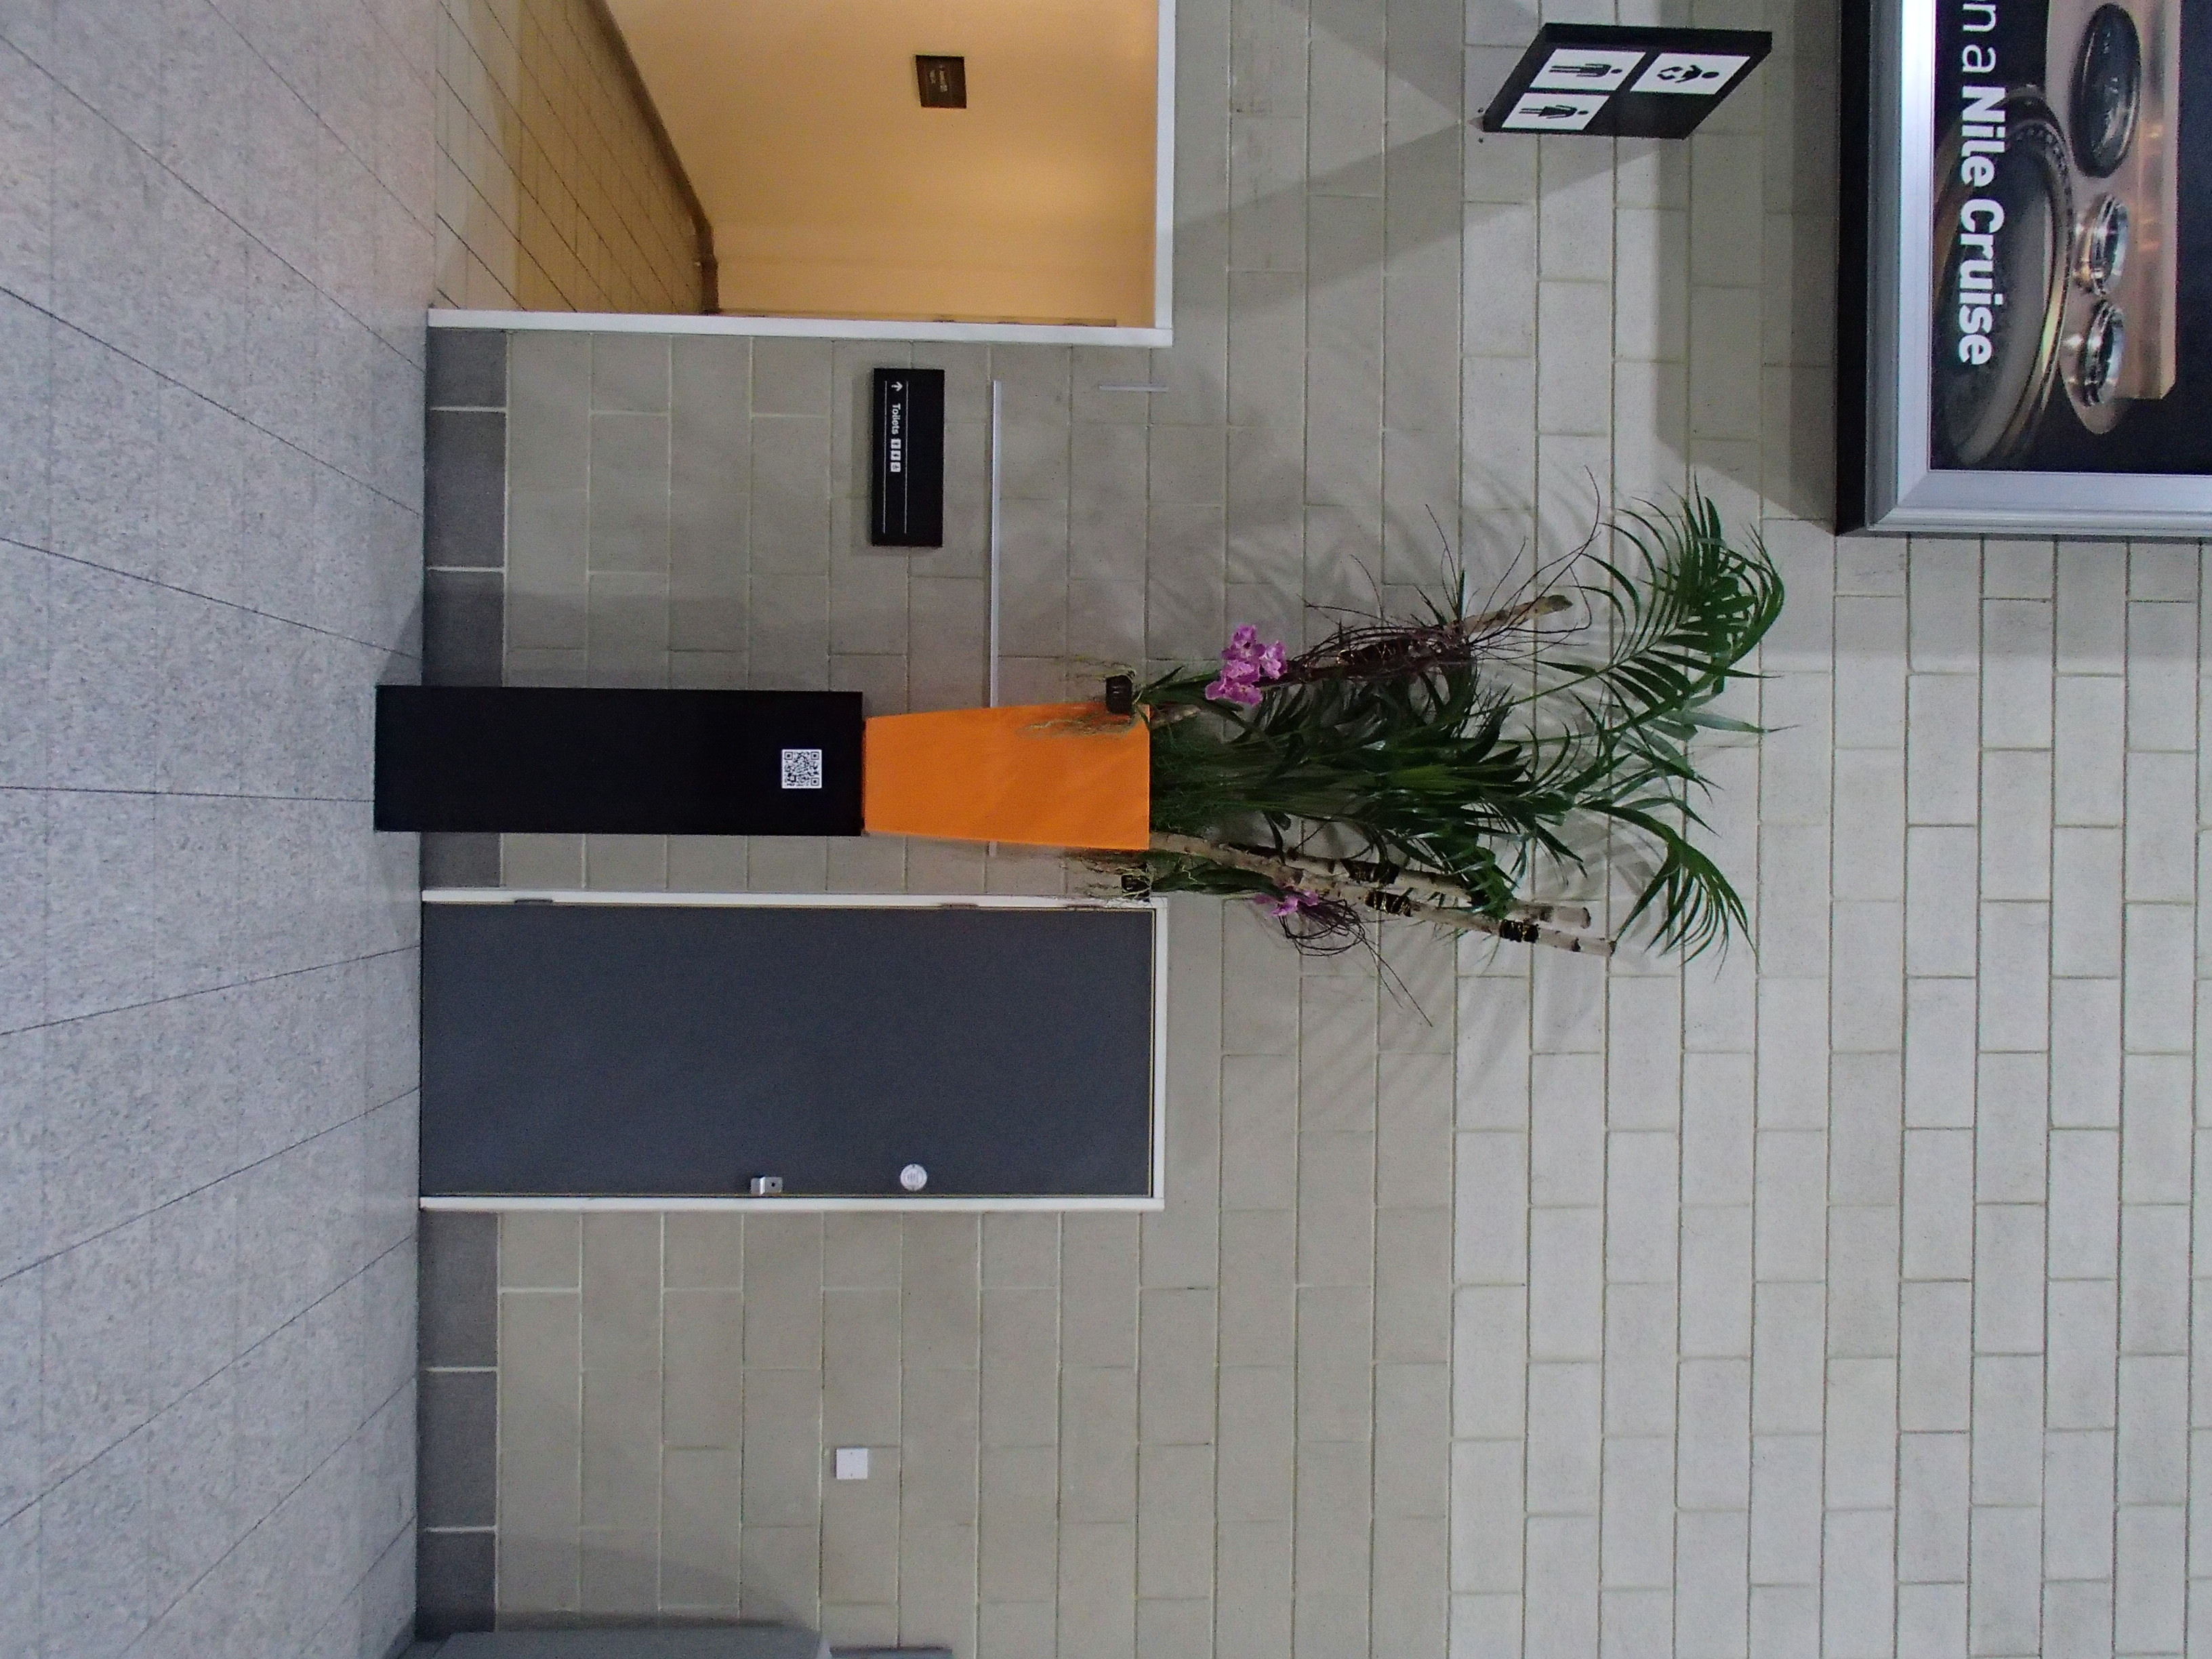
\includegraphics[width=\textwidth,angle=90]{figures/P1050143.JPG}
\caption{Plinth'd Nature}
\end{figure}

From a pedestal such as this one there is nothing further to be strived for but
full commune with the heavens. A small exemplar is chosen. Quickly, lightweight
channelling infrastructure is put in place, the thing is given an ``open top''.
Its delicate spread of antennae are placed out of arm's reach, the culturally
requisite lucky charms are added, disguised as decoration.

The base has wholly settled with the ground it sits on, happy to be so
possessed. This earthly protuberance that is relatively immovable plays host to
a spindly collection placed at the point where the thing gets as far as it
goes. From the simple guarantee of some weight something more contingent could
feel out (with imaginary hands) the safety to allow itself to emerge.

Simply put, this is technology manifest. A solid ``back box'' made of arcane
witchcraft lending stability to something otherwise intangible. Fragile human
emotion cradled gently by a larger process and so cradled allowed the space and
time to flourish generously to the delight of millions. There is almost a glow
about the thing, almost the sparkles of magic falling from its appendages. It
is how we know all is right with the world, we are in good company, we must be
cared for.

In this composition the perfect balance is struck in a sweep of asymmetry. An
image sails ahead unhanded and without guidance, forging a path of light and
leaving a spreading wake of shadows behind it. Standing in front of this
arrangement, this image of duality, the observer is thrown into a terrible and
relentless motion of their own. The coloured forms of the world shutter past at
pace, a cooling jet of histories and or of new ideas splashes on the brow and
spills away in dual rivers that meet between the shoulder blades. This is
motion without destination, as with ilynx and vertigo.

We see the expected, more human-scaled, more understandable artifacts of an
industrial construction; the visual clues that the thing as a whole did not
simply spring into existence, but rather came into being as the result of
repeated, tangential activity. The evidence appears as the side-effect of a
serious process, not as a direct mark. It arrives due to the necessity of
silencing the pleas for care and attendance from smaller details, and instead
lending favour to the needs of the larger work taking place.

We have an acute angle into another world, a tranche of matter is used as bait
for something much larger, something which looking from here is already vested
with some largesse and power. A brief and delicious salad snack to goad the
creeping and splintered advances of a richly different existence across to this
relatively poor one.

The structure here, this thing, should at any moment leap into brief, hideous,
frenetic action as the chanceless, raw power of the universe carves a bolt
across eons, through timeless permanence and permanence, just to be in touch
with an object that will be there \emph{one time only}. This thing is a ``one
shot'' fabrication designed to take a massive but fleeting single input.

There is nothing to see here close up, \emph{so we stand back}. Not one amongst
us wants to have his eyebrows singed by the power of the infinite.

\chapter{Nature in the 80s}

\begin{figure}
\centering
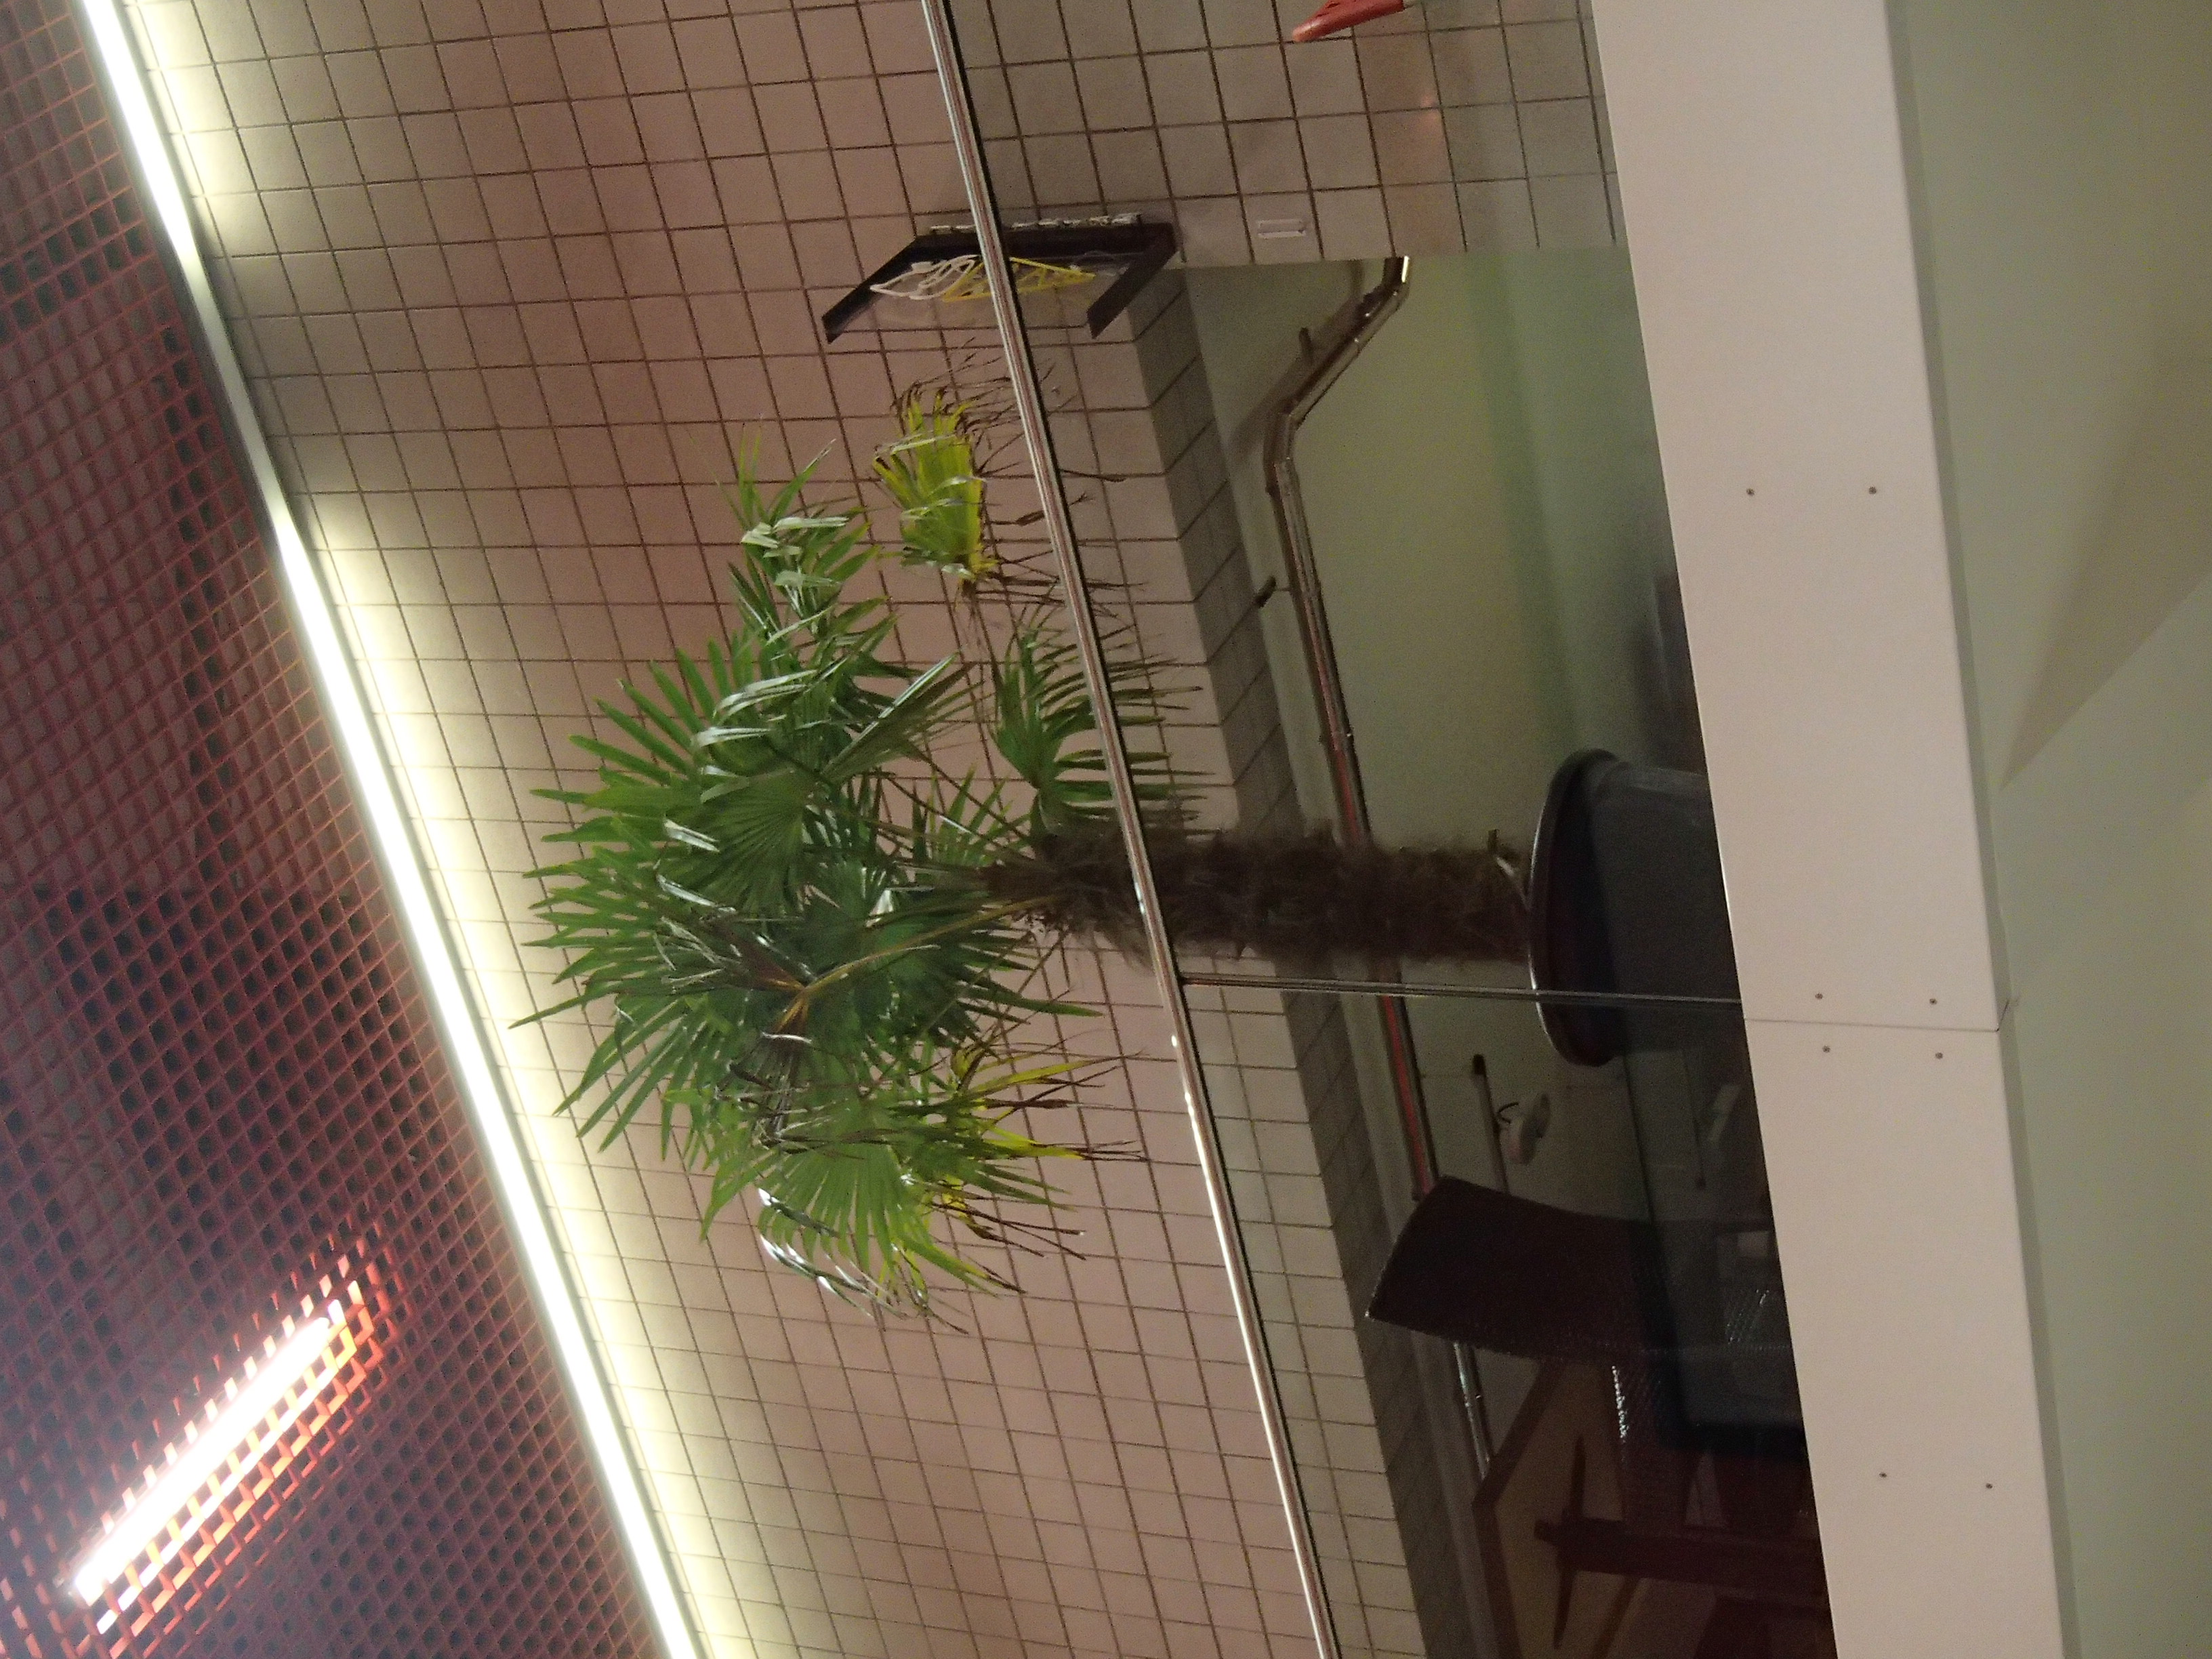
\includegraphics[width=\textwidth,angle=-90]{figures/P1050152.JPG}
\caption{Nature in the 80s}
\end{figure}

We don't remember what happened to us, just beginning to chase a new thought as
finance and oil exploded around us (in our midst). For a period nothing aged,
everything was \emph{as it was} and so it always would be. Our shared past, the
colloquial history of apes and animals was forgotten and cast aside in exchange
for this moment of shining clarity cast in shiny plastic.

At that time our human ``out-of-placeness'' became something commodifiable, the
hideous beast lurking within was invited (by advertising executives with wide
open arms and rather wild grins) to present itself publicly in lavish media
form, fully out in the world. In this gesture the animal in man became a
caricature of itself, greeting and hollering. It was left outside, pathetically
soliciting for encouragement and accepting any given.

Even money as we knew it ceased to have proper meaning, instead finance became
a kind of de facto government. We would never again have the same need to fish
or farm or struggle we once did, there would be pure opportunity for every man
to \emph{have} the things he desired; living, as he was, in a bizarre new
democracy of home furnishings and rubberised kitchen utensils.

All things people could own became in some sense red, white and blue without
anyone intending them to be. Where before wealth had distinct and well-defined
characteristics, now a new formal aesthetic began to develop, eschewing
decoration and detail for ergonomics and utilitarian elegance. The judgements
that for years could be made by studying the appearance of things suddenly
ceased to be hold water.  It became possible for validity to be built up and
broken down more quickly and by a greater proportion of the populous. So called
civil society changed size over night.

The pure scale upon which society operated was parabolically altered; the shape
of things sagged.

To those with humanity's brightening prospects in mind, humanity's prospects
were considerably brightened. Social mobility looked promising and desirable,
the swelling of classed people was good fun, technology was just great and all
these things empowered people. However, it is often forgotten in politics that
pure power will not dilute, it only switches polarity at a greater rate. So as
winds changed, the peaceful lacuna formed by something like time delay or lag
time was rapidly and harshly emptied. Its inhabitants found themselves strewn
broadly across a bleak, unforgiving landscape.

They found nothing like home, their quiet was replaced by the hum of fridges
and the low thundering of traffic. The peace they found in image was exposed as
mere impoverished understanding; hypnosis by the flickering of a television
screen, without proper appreciation for the real messages transmitted there.

Some stayed mobile, some just stayed. Maudlin denizens of a place that had had
its promise turned to ash. Now surrounded by bars and grids but still living,
seeming to the outside world all but montionless, making the quiet statement
\emph{``you don't have me like that''} by grimly singing low the songs of the
old country.

Indeed, some music could pass and stayed with them, but was only permitted to
pass when accompanied by proper documentation and even then only through
appropriate channels.

The world became too big and too empty and too flat, but these ex-regal figures
remained raised. They stood as weak beacons to their counterparts, thinly
sounding out a kind of stiff moisture against the overprescent smell of ozone.
In a scene of collapsing dust and the dry stains of ventilation they were the
small, shabby originals impossibly returning to their overblown simulacra.

We had no choice but to see them welcomed ``in'', there was too much sharing of
evolutionary roots; formal structure, growth patterns, etc. But, despite the
commonality, the two existed differently in time. One was nourished by its
passing and the other was slowly beaten back by it. The individual
relationships each shared with time essentially hid one from the by way of an
unassailable chasm of scale.

\chapter{Cornered Nature No. 1}
\label{chapter:cornered-nature-1}

\begin{figure}
\centering
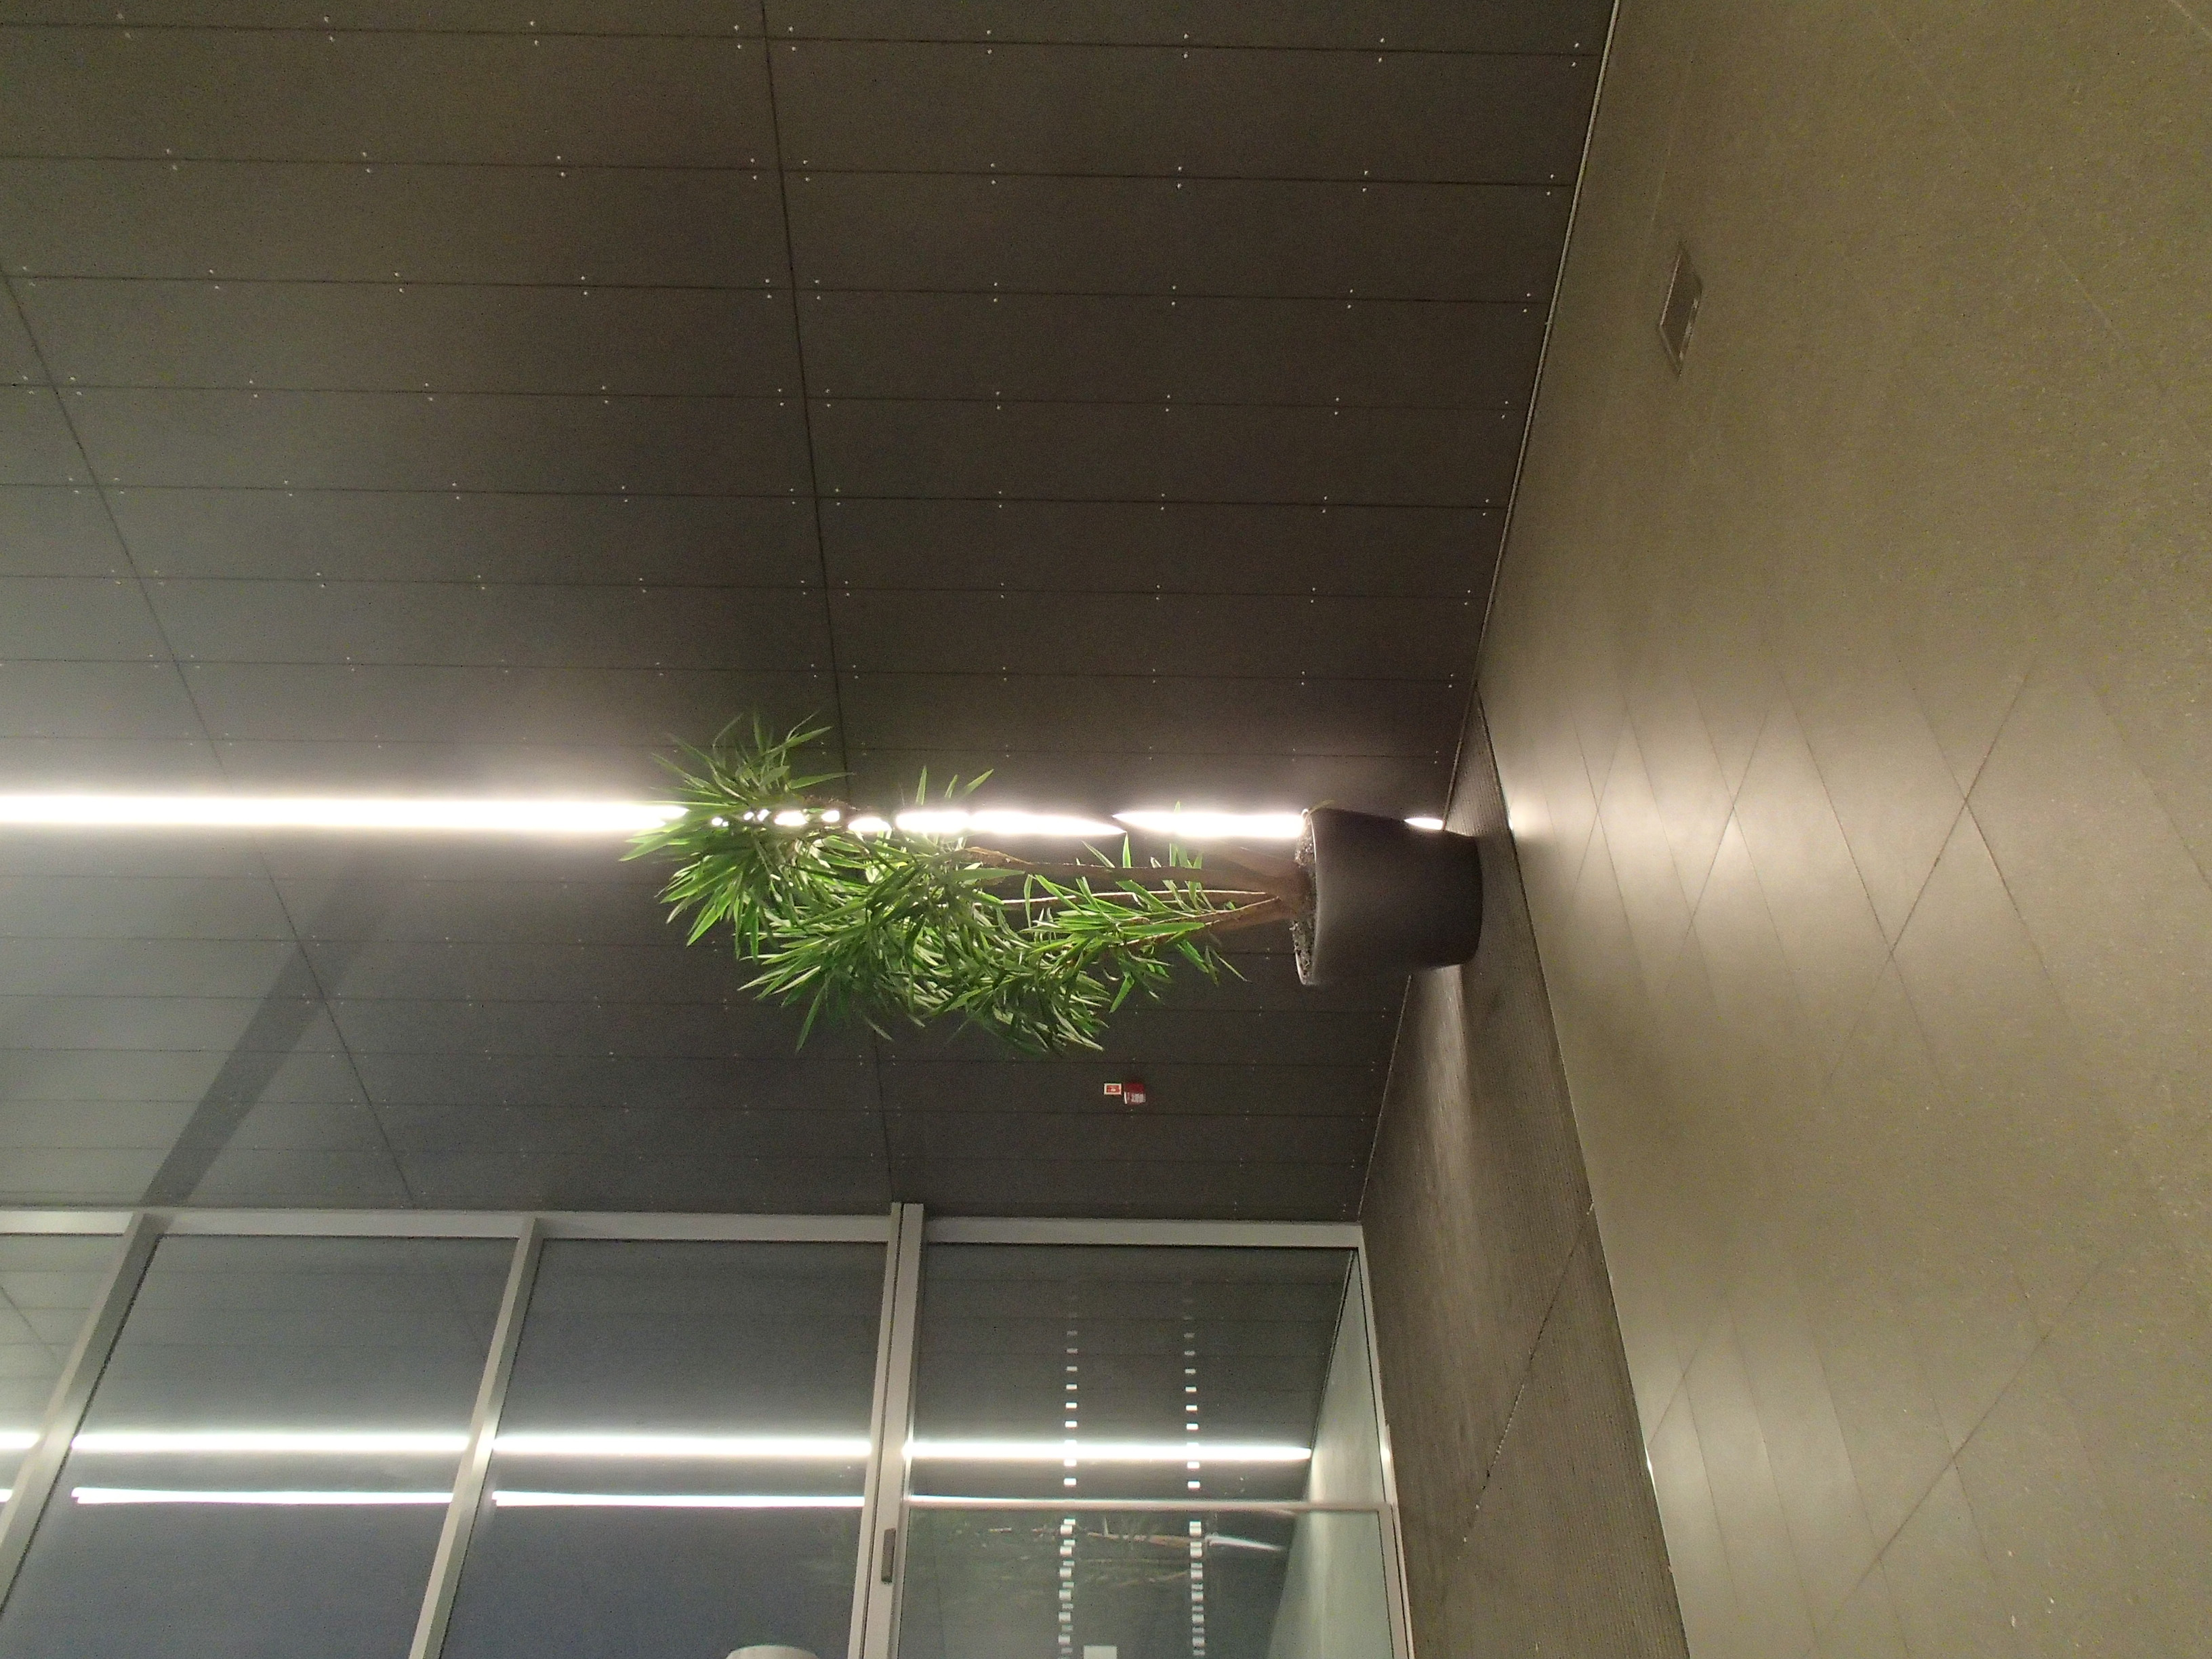
\includegraphics[width=\textwidth,angle=-90]{figures/P1050156.JPG}
\caption{Cornered Nature No. 1}
\end{figure}

Like most all defensive pretended misunderstanding, a body acting as if it
doesn't have any regard for its proper form is to be viewed as tragicomic for
sure, but more could be seen as possessing a strange heroism; it is engaged in
an odd battle against elegance.

Where the world flows smoothly, our hero jerks about. When surrounded by
ironed, filed receipts, our hero screws his own into crumpled balls and pockets
them. He refuses to see doorways, bumps into their jambs, trips on their stops
and swings on their hinges. At fancy restaurants he rudely smacks his lips and
tells dirty jokes on you, shouts at the staff, unkindly blows his nose on the
napkins.  On public transport he pushes and snarls, speaks too loudly, never
moves aside.  He leaps over the homeless in the street, does not respect the
traffic. He curses babies and children at any opportunity, leers at young
mothers, spits and snorts and smokes. He holds up queues and suddenly stops on
crowded pavements. He ignores email and will not answer the phone.

He is fighting powerfully, but the conditions necessary for his victory are
truly outlandish. How can one win a battle against the insurmountable by
attacking it with precisely the thing it was made to stand contrary to? Surely
impossible, with how the odds are stacked.

But there is a dream of the outside, or at least of somewhere to go. It may
take the throwing out of the baby with the bathwater; throwing everything else
away with the pain to get there, but there are no other options. Earlier in the
game something else could have happened (maybe something funny), but that time
is now past. A rock and an iron resolve holds each one exactly where she is, in
a life looking perfectly well like publicity material for something she might
buy to help with it.

No ticker-tape is promised, no piñata will be delivered. There is no officious
individual to hold the door or someone waiting for the opportunity to tell you
where to go. Only perhaps an Eastern plane of virgin space, a pine, buried
ceramics.

This is not a ham-fisted attempt to escape the condescension of Plato's cave,
it's nowhere near that complicated.  We are just moving from something we know
lots about and \emph{know} we don't like, to something that for a reason (that
for some reason Douglas Adams could never fathom) we know almost exactly
nothing about.

The strange thing is that all the things we \emph{do} know about where we are
trying to get to are not any of them things we don't like the sound of.

The percieved oddness of our hero can melt away. He is doing the only thing it
is conceivable to do in his situation; he sees the reality of where he is so
placed, but he will not admit to the unreality of what he is trying to do.

What he does not see is that through the lens of convention he has far exceeded
his goals; he is already ``from there''. His motion is so alien that he is
looked at not as an idividual standing in childish and pointless rebellion, but
as a telltale sign of serious and dreadful things to come, as though the
building will fall and slump to the ground as its foundations are revealed to
be made from green jelly.

\chapter{Cornered Nature No. 2}

\begin{figure}
\centering
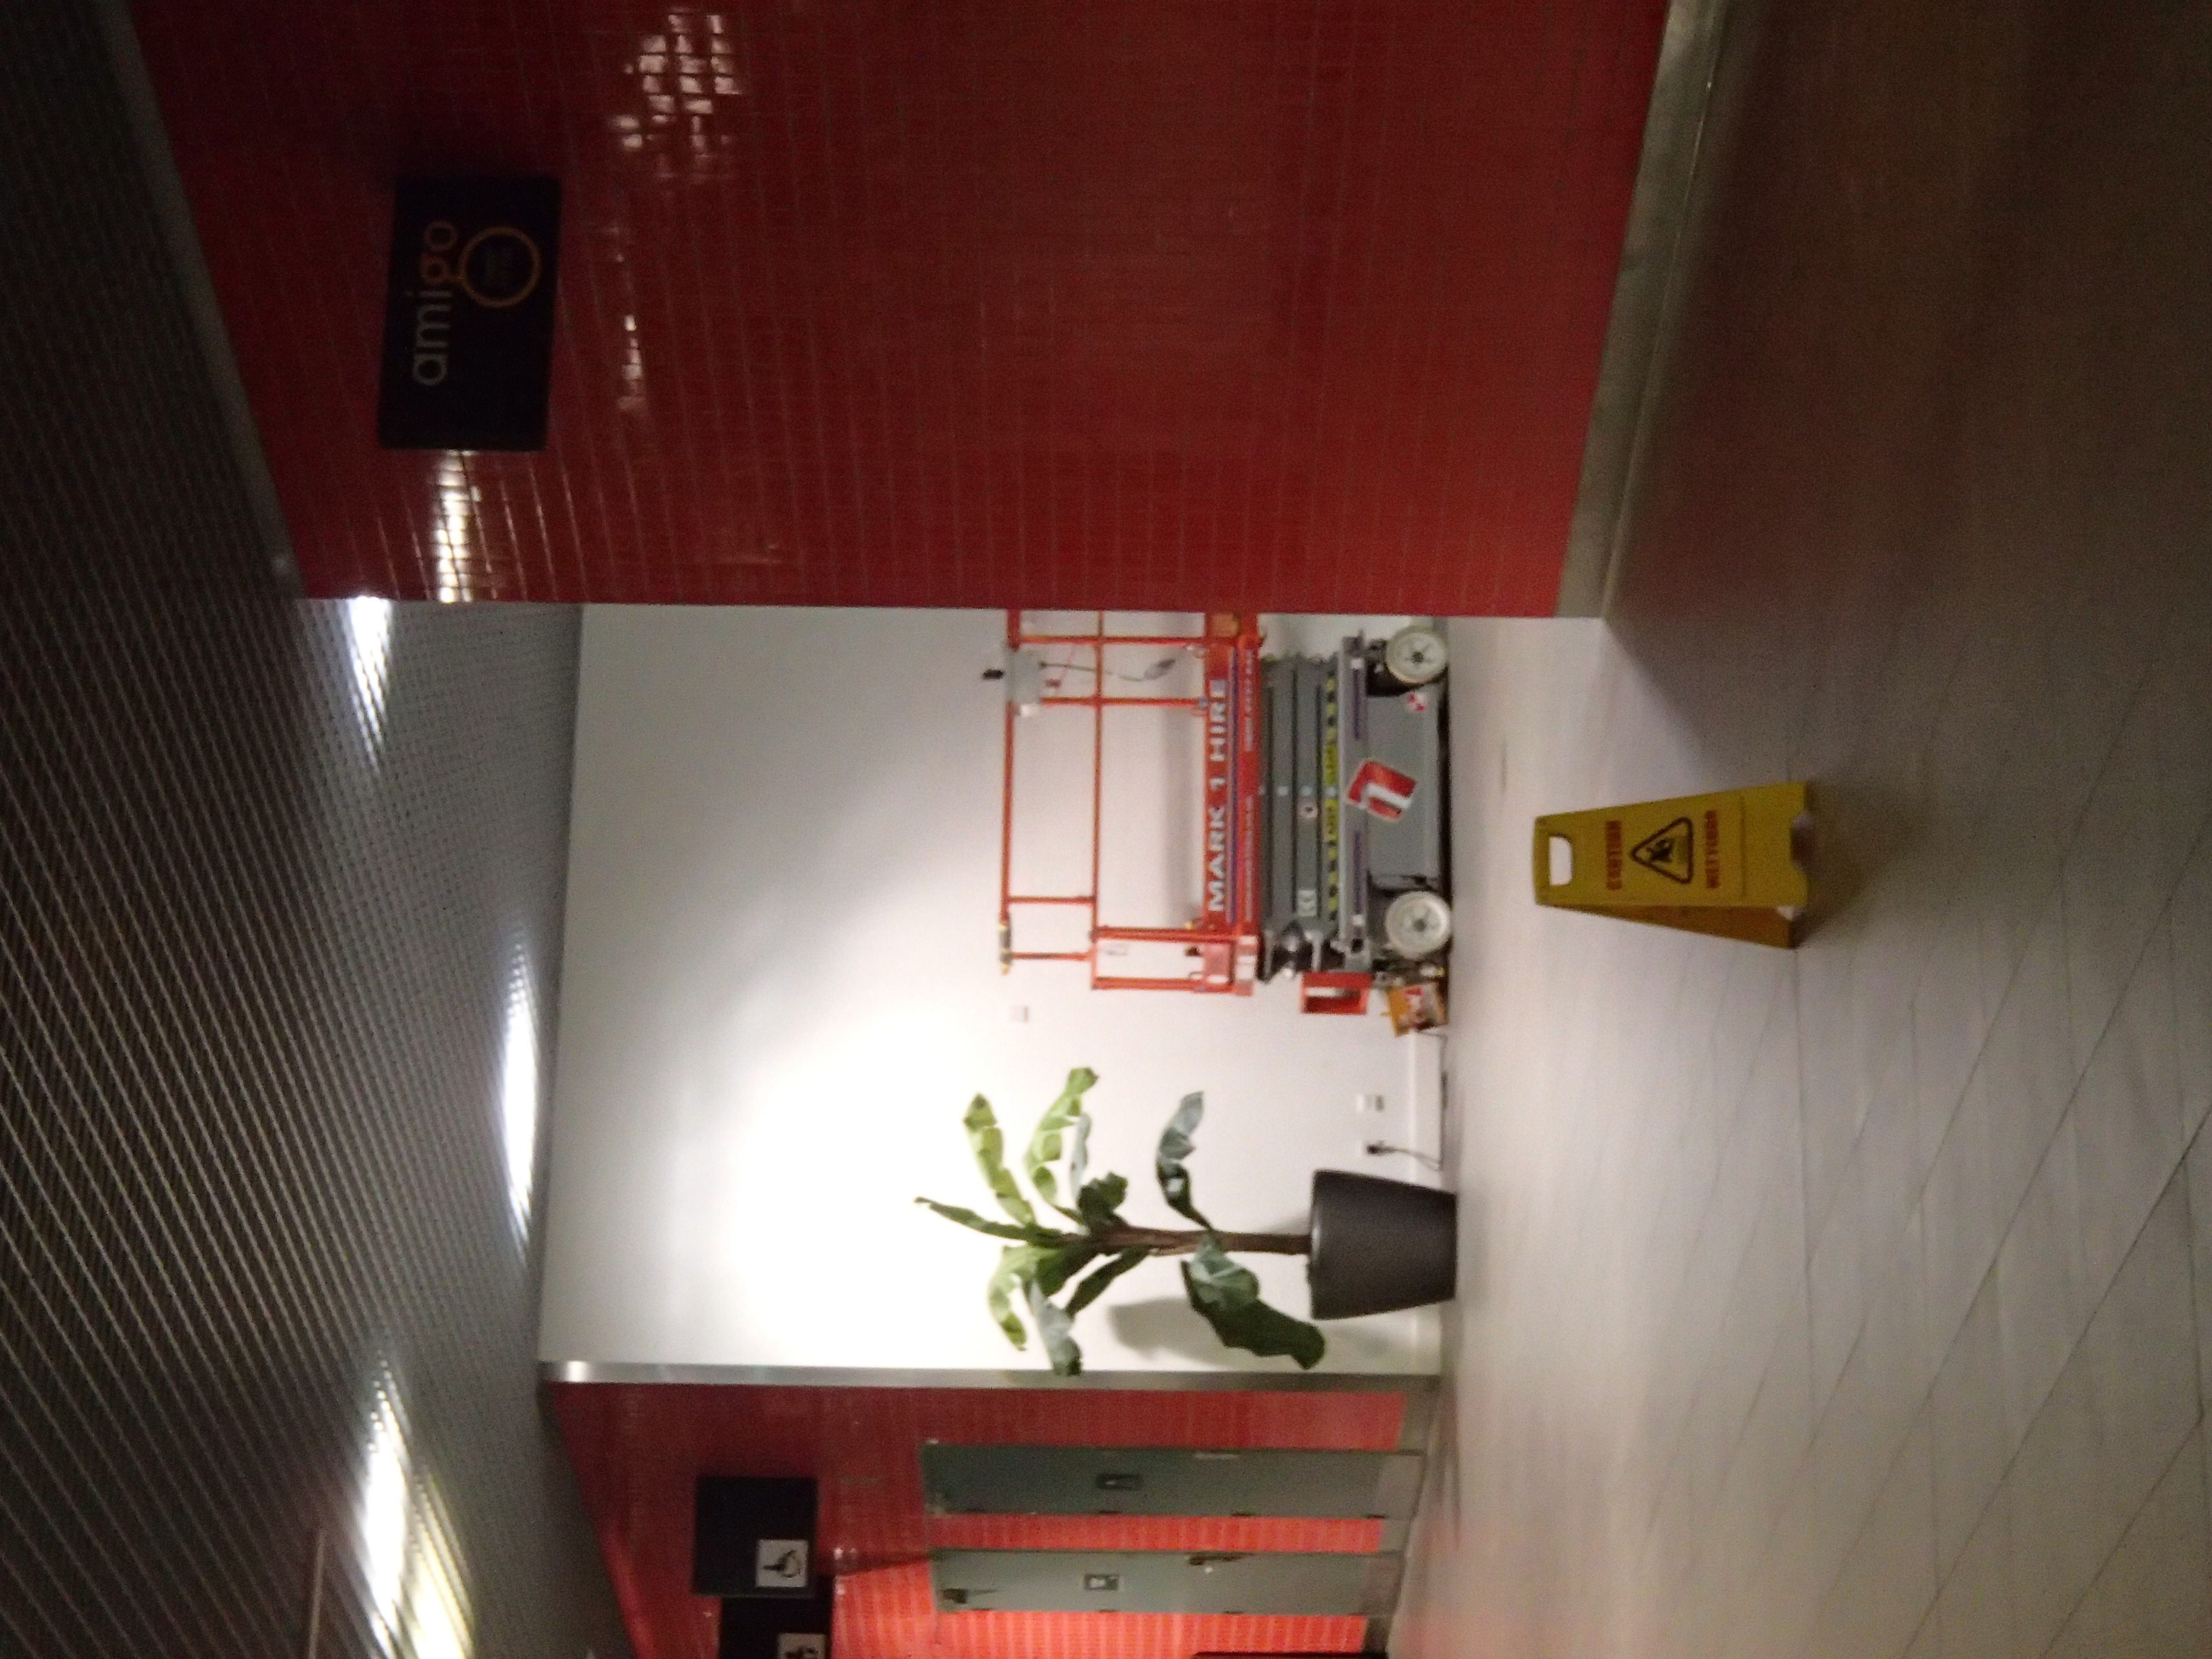
\includegraphics[width=\textwidth,angle=-90]{figures/P1050158.JPG}
\caption{Cornered Nature No. 2}
\end{figure}

Part of the magic of pre-made objects lies in their smugness; they appear to
have come from nowhere and seem to have always been there, they are rather
proud within themselves.

Seeing something that is so obviously prefab forces us to interrogate
everything else in the scene in order to find out what arrived on stage before
what.  Whatever the case, surely what we are is \emph{the late ones!} Thanks to
our very British and probably Victorian/Germanic propensity for imposing
grand narrative onto relative banality, it is precisely this accusatorial
question of chronology that bounds eagerly to the forefront of our
considerations.

We need to be able to point to the thing that naïvely fetched up amongst its
neighbours without the language to articulate exactly what its fetching up
could mean for either party. And conversely which thing arrived not strictly of
its own accord, fitting perfectly in, ``designed'' for some particular task or
set of purposes. Then we must ask how deeply considered this design. Designing
prefabricated objects is something like a game of chess.  We must try to see
how many moves ahead the designer was thinking, how long would we have to wait
until their intention is revealed by the purpose of the designed thing being
fulfilled?

With the off-kilter tone leaking from the initial question, we find ourselves
essentially (despite being presented with a clipped, polite arrangement),
considering which thing out of those before us is the most prefabricated. The
dumb things are set in a kind of competitive juxtaposition. They cannot profess
their innocence or admit their guilts (or, indeed, claim anything), they have
no exclamation to offer and so we can only judge on what we can see.

And shamefully, we find ourselves quickly organising, making an organisation,
assuming things are \emph{being done}. Because of the meaningful purpose imbued
in every shape and pattern (but for one), we can easily see what is \emph{being
done} (and to whom).

We have been a little bit silly in fostering this burning need to discover
which is more of the innocent party. All things are somewhat complicit in
their appearance.

\chapter{Nature Addendum}

\begin{figure}
\centering
\includegraphics[width=0.76\textwidth]{figures/20131116-1403-04.jpg}
\caption{Nature Addendum}
\end{figure}

A good fake is like a statement that abruptly diverts you from its stated
subject. It shortcuts through the long-winded formalities using an unexpected
(more ``lowly'', or completely other) formality. The thing presented is
wonderfully done; boasting smooth motion and perfect counterbalance, here
constructed entirely from sticks of bamboo, elastic bands and string; it
is such a brilliant idea that no one would actually think to do it.

It has its comedy too, like our hero from
Chapter~\ref{chapter:cornered-nature-1}, but the comedy here is expressed with
childlike mannerism. The portents our fake speaks of could be strikingly
ominous, but the language used to speak them simply lacks the gravitas afforded
by context to the original and so their messages are lost to babble (Bakhtin).

\end{document}
